%        File: report.tex
%     Created: Sat Nov 25 07:00 PM 2017 E
% Last Change: Sat Nov 25 07:00 PM 2017 E
%
\documentclass{article}
\usepackage{hyperref}
\usepackage{enumitem}
\usepackage{macros}

\usepackage[
backend=biber,
style=alphabetic,
bibencoding=ascii
]{biblatex}
\addbibresource{references.bib}

\usepackage{tikz}
\usetikzlibrary{math, arrows}

\title{Graph limits and Exchangeable Random Graphs}
\author{Miheer Dewaskar}


\begin{document}

\maketitle
\begin{abstract}
  This report explains dense-graph limits via graph statistics and exchangeable random graphs.
\end{abstract}

\section{Introduction}

Networks (and large networks) are ubiquitous in the real world. For instance, the human social network, about 7 billion nodes in size, determines the spread of ideas, news and diseases over the world. The human brain, which is a network of neurons, has about 100 billion nodes. And then of course there is the internet network, consisting of about 30 billion web-pages and probably more than a billion interconnected devices. With the advent of computers, our ambitions rose, and now we wish to understand these large networks. 

Graphs are mathematical models of networks and fundamental objects in discrete mathematics and computer science. Traditionally, lot of lot of efficient algorithms have been developed for graphs (shortest path, connectivity)  and computers today are fast as well. Despite this its not easy to deal with networks this large. Moreover we may not be interested in the exact quantities that traditional graph theory studies. For instance, consider the internet network. Does it make sense to ask if the internet is connected? Almost always, there will be some node which isn't connected. Moreover the internet network might not be exactly what it was a few minutes ago. But we may still be interested in quantities like the fraction of edges that need to be severed to divide the internet into two massive chunks. 

Such questions can be asked by sampling the network, and providing approximate answers to these questions quickly. The theory of graph limits that this report will dive into, develops the theory for sampling from large networks. But a caveat before we start: this theory is only useful for dense graphs (which a positive fraction of edges of the complete graph). See \cite{lovasz-book} for applications of the sampling methodology and further details.

\subsection{Notation}
\label{sec:notation}

Let $\N* \coloneqq \N \cup \set{\infty}$, $[n] \coloneqq \set{1,2,\dots,n}$ for $n \in \N$ and $[\infty] \coloneqq \N$.

A graph $G=(V,E)$ is a pair such that $V$ is a countable set of vertices and $E \subseteq V \times V$ is the set of edges. 
When only $G$ is given, $V(G)$ will denote the vertex set and $E(G)$ the edge set, and $v(G) = |V(G)|$. Without loss in generality, we can assume $V = [v(G)] \subseteq \N$ since $V$ is countable. We will consider undirected ($\forall u,v \in V \; (u,v) \in E \implies (v,u) \in E$) loop-free graphs ($\forall u \in V \; (u,u) \notin E$) only. Such a graph can be represented using graph diagrams as in \autoref{fig:example-graph}. 

$\Lg_{n}$ denotes the set of all (labeled) graphs on $[n]$ for any $n \in \N*$. For $n \in \N$, $\Lg_{n}$ has $2^{\binom{n}{2}}$ elements while $\Lg_{\infty}$ is uncountable. Let $\Lg \coloneqq \bigcup_{n \in \N} \Lg_{n}$ denote the set of all finite (labeled) graphs.
For $G_1, G_2 \in \Lg_{n}$, the relation $G_1 \subseteq G_2$ will denote the relation between the corresponding edge sets. 

Often, we are only interested in graphs up to a permutation of the vertices. That is, for $G, G' \in \Lg_{n}$ say $G \equiv G'$ if there is a permutation $\phi$ of $[n]$ so that $(i,j) \in E(G) \iff (\phi(i),\phi(j)) \in E(G')$. This is an equivalence relation, and its equivalence classes will denote unlabeled graphs. Hence formally, $\Ug_{n} \coloneqq \Lg_{n}/\equiv$ denotes the set of all unlabeled graphs on $[n]$ and $\Ug \coloneqq \bigcup_{n \in \N} \Ug_{n}$ is the set of all finite unlabeled graphs.

If $G$ is a finite graph and $v_1,\dots,v_k$ for $k \in \N$ is a sequence of vertices in $G$, then $G(v_1,\dots,v_k)$ denotes the labeled graph on vertex set $[k]$ where we put an edge between $i$ and $j$ if $(v_i, v_j) \in E(G)$. Note that we allow for vertices to repeat (if $v_i = v_j$ there there is no edge $(i, j)$ in $G(v_1, \dots, v_k)$).

We let $G[k]$, for $k \in \N$ be the random graph $G(V_1,\dots,V_k)$ obtained by sampling $V_1,\dots,V_k$ uniformly at random among the vertices of $G$ with replacement. Similarly, for $k \leq v(G) < \infty$, $G[k]'$ is the random graph $G(V'_1,\dots,V'_k)$ sampled uniformly at random without replacement. Hence $G[k]$ and $G'[k]$ are random graphs on $\Lg_{k}$ obtained from $G \in \Ug$. 


\begin{figure}
  \centering
  \begin{tikzpicture}[scale=.8]
    \tikzstyle{every node} = [circle]
    \node (a) at (0,0) {1};
    \node (b) at +(0:1.5) {2};
    \node (c) at +(60:1.5) {3};
    \foreach \from/\to in {a/b, b/c}
      \draw (\from) -- (\to);
  \end{tikzpicture}
  \caption{$G=(\set{1, 2, 3}, \set{(1,2), (2,1), (2,3), (3,2)})$}
  \label{fig:example-graph}
\end{figure}


\section{Convergence of graphs}
\label{sec:formal}
In this section we will embed $\Ug$ (finite unlabeled graphs) in a compact metric space. This will be done through graph statistics.

\subsection{Graph Statistic}

Fix a $G \in \Ug$. For $k \in \N$, $F \in \Lg_{k}$  define the graph statistic

\begin{equation}
  t(F, G) = \Pb(F \subseteq G[k])
  \label{eq:stat-def}
\end{equation}

This counts the proportion of all mapping $\phi : V(F) \to V(G)$ that are graph homomorphisms (i.e $(u, v) \in E(F) \implies (\phi(u), \phi(v)) \in E(G)$). See \cite[p.~6]{paper} which relates this to the number occurrences of $F$ in $G$, but working with graph homomorphisms is more convenient. Since the distribution of $G[k]$ is invariant under a change of labels, \eqref{eq:stat-def} only depends on the equivalence class of $F$. Hence we can assume that $t(F,G)$ is defined for $F \in \Ug_{k}$.  Using the inclusion-exclusion formula see that $(t(F, G))_{F \in \Ug_{k}}$ determine the distribution of $G[k]$. 

Now we explain how graph statistics $(t(F,G))_{F \in \Ug}$ preserve most of the information. First some notation:
\begin{align}
  \tau : \Ug &\to [0,1]^{\Ug} \nonumber\\
  \tau(G) &= (t(F, G))_{F \in \Ug}
  \label{eq:tau}
\end{align}
By the discussion above, if $\tau(G_1) = \tau(G_2)$  then $G_1[k] \dequal G_2[k] \; \forall k \in \N$.
In addition if $v(G_1) = v(G_2) = n$, then by induction we can show $G_1'[k] = G_2'[k] \; \forall k \leq n$. Taking $k=n$, since $G_i'[n] \equiv G_i$, shows that $G_1 \equiv G_2$. Hence $\tau$ is injective on $\Ug_{n}$. 

But $\tau$ is not injective in general. For a graph $G$ and any $k \in \N$ consider the $r$-blowup $G_r=(V,E)$ with vertex set $V = V(G) \times [r]$ and edges $E=\set{((u, i), (v, j)) \mid (u,v) \in E(G), i,j \in [r]}$ (see \autoref{fig:blowup}). Then  $G[k] \dequal G_r[k] \; \forall k \in \N$ and hence $\tau(G) = \tau(G_r)$. To alleviate this we define
\begin{align}
  \tau^+ : \Ug &\to [0,1]^{\Ug} \times [0, 1] \nonumber \\
  \tau^+(G) &= \left(\tau(G), v(G)^{-1}\right)
  \label{eq:embedding}
\end{align}
Thus $\tau^+$ embeds $\Ug$ into the space $[0,1]^{\Ug+} \coloneqq [0,1]^{\Ug}\times [0,1]$. 


\begin{figure}
  \centering
  \tikzstyle{every node}=[circle, draw, fill=black!50,
                        inner sep=0pt, minimum width=4pt]
  \begin{tikzpicture}[scale=2]
    \node (a) at (0,0) {};
    \node (b) at +(0:1) {};
    \node (c) at +(60:1) {};
    \foreach \from/\to in {a/b, b/c}
      \draw (\from) -- (\to);
  \end{tikzpicture} \quad 
  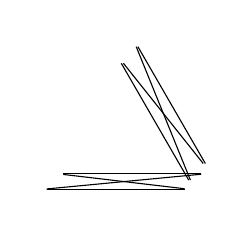
\begin{tikzpicture}[scale=2]
    \foreach \k in {1,2} {
      \path[xshift=\k*3pt, yshift=\k*3pt] (0,0) node (a\k) {} -- +(0:1) node (b\k) {} +(60:1) node (c\k) {};
    }
    \foreach \from/\to in {a/b, b/c} 
      \foreach \k in {1,2}
       \foreach \l in {1,2}
        \draw (\from\k) -- (\to\l);
  \end{tikzpicture}
  \caption{Graph and its 2-blowup}
  \label{fig:blowup}
\end{figure}


\subsection{Graph limits}

The graph limit theory developed in \cite{lovasz04} states that a sequence of graphs $\left( G_n \right)_{n \in \N} \subseteq \Ug$ converge if $\tau(F, G_n)$ converge for every $F \in \Ug$ or equivalently if the sequence of random graphs $(G_n[k])_{n \in \N}$ on $\Lg_{k}$ converge in distribution for every $k \in \N$. An example of this convergence is given next.

\newcommand{\p}{0.5}
\begin{example}
  \label{ex:convergence}
  Consider the function $W: [0,1] \times [0,1] \to [0,1]$ given below (defined almost everywhere):

  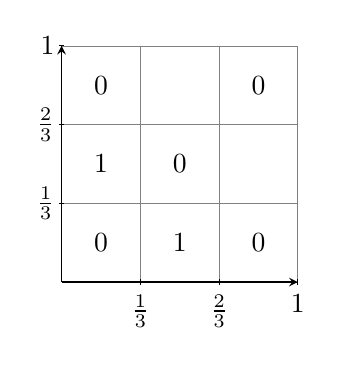
\begin{tikzpicture}[scale=1, >=stealth]
    \draw[step=, help lines] (0,0) grid (3,3);
    \draw[->] (0,0) -- (3,0);
    \draw[->] (0,0) -- (0, 3);
    \foreach \x/\xtext in {1/\frac{1}{3},2/\frac{2}{3},3/1}
      \draw (\x, 1pt) -- (\x, -1pt) node[below] {$\xtext$};
    \foreach \y/\ytext in {1/\frac{1}{3},2/\frac{2}{3},3/1}
      \draw (-1pt, \y) -- (+1pt, \y) node[left] {$\ytext$};

      \begin{scope}[shift={(-0.5cm, -0.5cm)}]
      % off diagonal
      \foreach \x/\y/\val in {1/2/1, 1/3/0, 2/3/\p}
      {
	\node at (\x, \y) {$\val$};
	\node at (\y, \x) {$\val$};
      }
      % diagonal
      \foreach \x/\val in {1, 2, 3}
	\node at (\x, \x) {$0$};
    \end{scope}
  \end{tikzpicture}

  For $n \in \N$, generate graph a graph $G_n \in \Lg_{n}$ as follows: sample $U_1,\dots,U_n$ i.i.d $U[0,1]$ and connect nodes $i < j \in [n]$ with probability $W(U_i, U_j)$ independent of all other pair of nodes. Then by \cite[p.~185]{lovasz-book}, the resulting $G_n$ converge (as $n \to \infty$) with probability 1 and the limit can be identified with $W$. 

  This was a way to generate graphs with both structure and randomness. \autoref{fig:convergence} provides a visual interpretation of the convergence (which is formalized using the cut metric \cite[p.~127]{lovasz-book}).
\end{example}

\begin{figure}
  \centering
  \begin{tikzpicture}[scale=1.5, 
      ]
    \draw[dotted] (0,0) circle (.5);
    \draw[dotted] (60:2) circle (.5);
    \draw[dotted] (0:2) circle (.5);

   \pgfmathsetmacro{\n}{5}
   \pgfmathsetmacro{\p}{\p}
   \newcommand{\point}[1]{(360*\k/\n:.3)}

   \begin{scope}[every node/.style={circle, fill=black!50,
     inner sep=0pt, minimum width=4pt}, very thin]
     \foreach \k in {1,...,\n} 
       \path (0,0) +\point{\k} node (a\k) {} (60:2) +\point{\k} node (c\k) {} (0:2) +\point{\k} node (b\k) {}; 
     \foreach \k in {1,...,\n}
       \foreach \m in {1,...,\n} {
	\draw (a\k) -- (b\m);
	\pgfmathparse{(1+rand)/2 < \p}
	\ifnum\pgfmathresult=1 
	  \draw (b\k)--(c\m);
	\fi
      }
   \end{scope}
   \draw[->, >=stealth, double] (3,1) -- (4,1) node[pos=.5, above] {$n \to \infty$};

   \begin{scope}[xshift=5cm, vertex/.style={circle, minimum width=.5cm, draw}]
     \draw (0,0) node[vertex] (a) {$\frac{1}{3}$};
     \draw (60:2) node[vertex] (c) {$\frac{1}{3}$};
     \draw (0:2) node[vertex] (b) {$\frac{1}{3}$};
     \draw (a) -- (b) node[above, pos=.5] {$1$};
     \draw (b) -- (c) node[above right, pos=.5] {$\p$};
   \end{scope}
  \end{tikzpicture}

\caption{Graphs on $n$ vertices converging to a limit.}
  \label{fig:convergence}
\end{figure}

To formalize this concept of limit we identify $\Ug$ with the topological space $\tau^{+}(\Ug)$. Let $\Ug*$ be the closure of $\Ug$ in $[0,1]^{\Ug^+}$, and denote by $\Ug_{\infty} \coloneqq \Ug*\setminus \Ug$. Observe that 
\begin{enumerate}
  \item $\Ug_{\infty} = \Ug* \cap  \left( [0,1]^{\Ug}\times \set{0} \right)$ as so $\Ug_\infty$ is closed.
  \item $\Ug_{\infty} = \overline{\tau(\Ug)} \times \set{0}$ since $\tau$ is constant on blowups. 
\end{enumerate}

Hence $\Ug_{\infty}$ can be identified with the graph limits $\overline{\tau(\Ug)}$. In particular every $G \in \Ug$ is associated with a ghost $\tau(G)$ in $\Ug_{\infty}$. Both $\Ug*$ and $\Ug_{\infty}$ are closed subsets of $[0,1]^{\Ug^+}$ and hence compact. The graph statistics $\tau(\cdot) = (t(F, \cdot))_{F \in \Ug}$ continuously (and uniquely) extend from $\Ug$ to $\Ug*$. Then $\tau$ is injective on $\Ug_{n}$ for any $n \in \N*$. Similarly extend $v$ by defining $v(G) = \infty$ on $\Ug_{\infty}$ so that each element $G \in \Ug*$ is just $\left( \tau(G), v(G)^{-1} \right) \in [0,1]^{\Ug^+}$.
 

We end this section with a lemma.

\begin{lemma}
  \label{lem:disjoint}
  For any $G \in \Ug*$ and $F_1, F_2, \ldots, F_k \in \Ug$ 
  \begin{equation}
    t(\Oplus_{j=1}^k F_j, G) = \prod_{j=1}^k t(F_j, G)
    \label{eq:tdirectsum}
  \end{equation}
  where $\Oplus_{j=1}^k F_j \in \Ug$ is the graph corresponding to disjoint union of $F_j$'s.
\end{lemma}
\begin{proof}
  By continuity of the graph statistics we just need to show this for $G \in \Ug$. 

  Let $F = \Oplus_{j=1}^k F_j \in \Lg_{n}$. For $1 \leq j \leq k$, let $I_j \subseteq [n]$ be the vertices in $F$ corresponding to $F_j$ and assume $V_1,\dots, V_n$ is an i.i.d sample from $V(G)$.
  \begin{align*}
    t(F, G) &= \Pb(\Oplus_{j=1}^k F_j  \subseteq G(V_1,\dots,V_n)) \\
    &= \Pb(\bigcap_{j=1}^k \set{F_j \subseteq G((V_i)_{i \in I_j})}) \\
    \shortintertext{since $I_j$ are disjoint use independence of $V_i$}
    &= \prod_{i=1}^k \Pb(F_i \subseteq G((V_i)_{i \in I_j})) = \prod_{i=1}^k t(F, G)
  \end{align*}
\end{proof}

\subsection{Random Graphs}

In this section we will analyze random elements and weak convergence in $\Ug*$. Since we have already embedded it in $[0,1]^{\Ug^+}$ not much needs to be done to get the next theorem (from \cite{paper})

\begin{theorem}
  \label{thm:dconv-graph}
  Let $(G_n)_{n \in \N}$ be a sequence of random elements in $\Ug*$ with $v(G_n) \pconv \infty$. Then the following are equivalent as $n \to \infty$.
  \begin{enumerate}[label=(\roman*)]
    \item $G_n \dconv \Gamma$ for some random $\Gamma \in \Ug*$ \label{itm:1}
      \item For every finite family $F_1, F_2 \ldots, F_m \in \Ug$ of (non-random) graphs, the random variables $t(F_1, G_n),\dots,t(F_m,G_n)$ converge jointly in distribution.\label{itm:2}
      \item For every (non-random) $F \in \Ug$, the random variables $t(F, G_n)$ converge in distribution.\label{itm:3}
      \item For every (non-random) $F \in \Ug$, the expectations $\Ex[ t(F, G_n) ]$ converge.\label{itm:4}
    \end{enumerate}
    If these properties hold, then the limits in \ref{itm:2}, \ref{itm:3} and \ref{itm:4} are $\left( (t(F_i, \Gamma) \right)_{i=1}^m$, $t(F, \Gamma)$ and $\Ex[ t(F, \Gamma) ]$, respectively. Furthermore, $\Gamma \in \Ug_{\infty}$ a.s
\end{theorem}
\begin{proof}
  $\ref{itm:1} \iff \ref{itm:2}$ Since $\Ug*$ is a closed subset of $[0,1]^{\Ug^+}$, convergence in distribution in $\Ug*$ is equivalent to convergence of $\tau^+(G) = \left( (t(F, G_n))_{F \in \Ug}, v(G_n)^{-1} \right)$ in $[0,1]^{\Ug^+}$. Since we assume $v(G_n)^{-1} \pconv 0$, this is equivalent to convergence of $\left( t(F, G_n) \right)_{F \in \Ug}$ in $[0,1]^{\Ug}$ (\cite{weak-conv}[Theorem 4.4]), which is equivalent to convergence of all finite families $(t(F_i, G_n))_{i=1}^m$ (\cite{weak-conv}[p.~19]). 

  $\ref{itm:2} \implies \ref{itm:3}$ Trivial.

  $\ref{itm:3} \implies \ref{itm:4}$ Immediate since $t$ is bounded by 1.

  $\ref{itm:4} \implies \ref{itm:2}$ Let $F_1, \dots, F_m \in \Ug$. For any $l_1,\dots,l_m \in \N$ construct a graph $F$ which is a disjoint union of $l_1$ copies of $F_1$, $l_2$ copies of $F_m$ and so on. If \ref{itm:4} holds then $\Ex[ t(F, G_n) ]$ converge. Hence by \autoref{lem:disjoint} 
  \begin{equation}
    \lim_{n \to \infty}E{\prod_{i=1}^m t(F_i, G_n)^{l_i}}
    \label{eq:moments}
  \end{equation}
  exists for every $l_1,\dots, l_m \in \N$. Since the graph statistics are all bounded by the method of moments $(t(F_1, G_n),\dots, t(F_m, G_n))$ converges jointly in distribution.
  Since $v(G_n)^{-1} \pconv 0$, $v(\Gamma)^{-1} = 0$ and so $\Gamma \in \Ug_{\infty}$ almost surely. Once we know that $G_n \dconv \Gamma$ then limits in \ref{itm:2}, \ref{itm:3}, \ref{itm:4} are as described.
\end{proof}

\begin{cor}
  \label{cor:dconv8}
  If $(\Gamma_n)_{n \in \N}$ is a sequence of random elements in $\Ug_{\infty}$ then $(\Gamma_n)_{n \in \N}$ converge in distribution to a random element $\Gamma \in \Ug_{\infty}$ if and only if $\lim_{n \to \infty} \Ex t(F, \Gamma_n) = \Ex t(F, \Gamma)$ for every $F \in \Ug$.
\end{cor}
\begin{proof}
  In \autoref{thm:dconv-graph} take $G_n=\Gamma_n$ since $v(\Gamma_n) = \infty$.
\end{proof}
\begin{cor}
  The distribution of a random element $\Gamma \in \Ug_{\infty}$ is uniquely determined by $\left(\Ex t(F, \Gamma)\right)_{F \in \Ug}$
\end{cor}
\begin{proof}
  Take $\Gamma_n = \Gamma$ in \autoref{cor:dconv8}.
\end{proof}

\section{Graph limits and exchangeable random graphs}
\label{sec:sampling-distribution}

In the previous section we formally constructed a compact metric space $\Ug*$ and the space $\Ug_{\infty}$ of graph limits. We also examined weak-convergence of $\Ug_{\infty}$ valued random elements. In this section we will see (\autoref{thm:corres}) another representation for probability measures on $\Ug_{\infty}$ in terms of exchangeable probability measures on $\Lg_{\infty}$.

\subsection{Infinite Graphs}

In this section we will look at graphs with vertex set $\N = \set{1, 2, 3, \ldots}$.  The set of all such graphs is denoted by $\Lg_{\infty}$. These graphs are determined by their edge set hence $\Lg_{\infty}$ can be identified by $\set{0,1}^{E(K_{\infty})}$ where $K_\infty$ is the complete graph on $\N$. We give this space (and thus $\Lg_{\infty}$) the product topology. Hence $\Lg_{\infty}$ is a compact metric space.

Sometimes we will associate a $G \in \Lg_{n}$ with an infinite graph obtained by adding isolated vertices for $\set{n+1, n+2, \ldots}$. For $H \in \Lg_{\infty}$ the restriction operation $\restr{H}{[k]} = H(1,\dots,k)$ will denote the induced subgraph (in $\Lg_{k}$) on vertices $[k]$. 

For a finite graph $G$, we can also define the sampling graph $G[\infty]$ by taking an i.i.d random sample $V_1, V_2,\cdots$ from $V(G)$ and defining $G[\infty] \coloneqq G(V_1, V_2, \ldots)$ to be the random graph (in $\Lg_{\infty}$) induced by these vertices. Note that the random graphs $G[k]$ for $k \in \N$ satisfy $G[k] \dequal \restr{G[\infty]}{[k]}$. And since the topology on $\Lg_{\infty}$ is the product topology on $\set{0,1}^{E(K_\infty)}$, any random graph $H \in \Lg_{\infty}$ uniquely determined by its distributions $\restr{H}{k}$ on $\Lg_{\infty}$. Moreover for random graphs $H_n \in \Lg_{\infty}$, $H_n \dconv H \in \Lg_{\infty}$ if and only if $\restr{H_n}{[k]} \dconv \restr{H}{k}$ for every $k \in \N$.

If $G$ is a finite graph, let $\h{G}$ denote the finite graph obtained by randomly labeling the vertices of $G$ by $1,\dots, v(G)$. In other words $\h{G} = G[v(G)]$ is a random graph on $\Lg_{v(G)}$.  We will at times consider this as a random graph on $\Lg_{\infty}$ as mentioned above. The thing to note is the as $v(G) \to \infty$ for any $k \in \N$, $\restr{\h{G}}{k}$ has nearly the same distribution as $G[k]$. Note this while trying to understand \autoref{thm:constr} along with the following comment.

As a motivation for what follows, let us look at a (non-random) sequence of graph $(G_n)_{n \in \N} \subseteq \Ug$ with $v(G_n) \to \infty$. Then $t(F, G_n) = \Pb(F \subseteq G_n[k])$ converge for every $F \in \Ug$ if and only if for all $k \in \N$, $G_n[k] \dconv \cdot $ and equivalently $G_n[\infty] \dconv \gamma$ for some random graph $\gamma \in \Lg_{\infty}$. This construction associates a random infinite graph $\gamma$ to every graph limit. \autoref{thm:constr} shows that this construction extends to random elements in the space of graph limits ($\Ug_{\infty}$) and will finally \autoref{thm:corres} be used to show a one-to-one correspondence between distributions on graph limits and class of random graphs on $\Lg_{\infty}$.

\begin{theorem}[{\cite{paper}[Theorem~4.1]}]
  \label{thm:constr}
   Let $\left( G_n \right)$ be a sequence of random graphs in $\Ug$ and assume that $v(G_n) \to \infty$. Then the following are equivalent.
  \begin{enumerate}
    \item $G_n \dconv \Gamma$ in $\Ug*$ for some random variable $\Gamma \in \Ug*$
    \item $G_n[\infty] \dconv H$ in $\Lg_{\infty}$ for some random $H \in \Lg_{\infty}$
    \item $\h{G_n} \dconv H$ in $\Lg_{\infty}$ for some random $H \in \Lg_{\infty}$
  \end{enumerate}
  If these hold, then $\Pb(F \subseteq \restr{H}{[k]}) = \Ex[t(F, \Gamma)]$ for every $F \in \Lg_{k}$. Furthermore, $\Gamma \in \Ug_{\infty}$ a.s
  \label{thm:conv-to-infinite-graphs}
\end{theorem}

\subsection{Exchangeable random graphs}
\begin{definition}
  A random graph $H \in \Lg_{\infty}$ is said to be \emph{exchangeable} if its distribution is invariant under every permutation of vertices. 
\end{definition}

It is actually sufficient to check that the distribution of $H$ is invariant under finite permutations, i.e any permutation $\phi: \N \to \N$ so that $\set{i | \phi(i) \neq i}$ is finite. This is because joint distributions are determined by finite dimensional distributions.

\begin{lemma}
  \label{lem:exch}
  Let $H$ be a random infinite graph in $\Lg_{\infty}$. Then the following are equivalent
  \begin{enumerate}[label=(\roman*)]
    \item $H$ is exchangeable.
    \item $\restr{H}{[k]}$ has a distribution invariant under all permutations of $[k]$ for every $k \geq 1$.
    \item $\Pb(F = \restr{H}{[k]})$ depends only on the isomorphism type of $F$, and can thus be seen as a function of $F$ as an unlabeled graph in $\Ug_{k}$ for every $k \geq 1$.
  \end{enumerate}
\end{lemma}

\begin{theorem}[{\cite{paper}[Theorem~5.3]}]
  \label{thm:corres}
  There is one-to-one correspondence between distributions of random elements $\Gamma \in \Ug_{\infty}$ and distributions of exchangeable random graphs $H \in \Lg_{\infty}$ given by
  \begin{equation}
    \Ex t(F, \Gamma) = \Pb(F \subseteq \restr{H}{[k]})
    \label{eq:corres}
  \end{equation}
  for every $k \geq 1$ and $F \in \Lg_{k}$. Furthermore $\restr{H}{[n]} \dconv \Gamma$ in $\Ug*$ as $n \to \infty$.
\end{theorem}

\begin{cor}
  The correspondence in \autoref{thm:corres} is a homeomorphism.
\end{cor}
\begin{proof}
  Suppose $H_n \sim \Gamma_n$ and $H \sim \Gamma$ where $(H_n)_{n \in \N}, H$ are random graphs in $\Lg_{\infty}$ and $(\Gamma_n)_{n \in \N}, \Gamma$ are random elements in $\Ug_{\infty}$.
  As we have stated, $H_n \dconv H$ in $\Lg_{\infty}$ if and only if for every $k \geq 1$, $\restr{H_n}{[k]} \dconv \restr{H}{[k]}$.
  Similarly by \autoref{cor:dconv8} $\Gamma_n \to \Gamma$ if and only if for every $F \in \Ug$, $\Ex t(F, \Gamma_n) \to \Ex t(F, \Gamma)$. Hence combining this with \eqref{eq:corres}, we get $\Gamma_n \dconv \Gamma$ if and only if $H_n \dconv H$.
\end{proof}
\begin{cor}
  \label{cor:extreme-corres}
  \autoref{thm:corres} gives a one-to-one correspondence between elements $\Gamma$ of $\Ug_{\infty}$ and the extreme points of the set of distributions of exchangeable random infinite graphs $H \in \Gamma$. This correspondence is given by
  \begin{equation}
    t(F, \Gamma) = \Pb(F \subseteq \restr{H}{[k]})
    \label{eq:extreme-corres}
  \end{equation}
  for every $F \in \Lg_{k}$. Furthermore, $\restr{H}{n} \xrightarrow{a.s} \Gamma$ in $\Ug*$ as $n \to \infty$.
\end{cor}
\begin{proof}
  The extreme points of the set of distributions on $\Ug_{\infty}$ are point masses. Since the correspondence from \eqref{eq:corres} is affine (in the space of probability measures on both sides), the extreme points must be in correspondence with each other. 
\end{proof}

\section{Conclusion}

In \autoref{sec:formal} we formally embedded the set of unlabeled graphs in a compact metric space using the graph statistics \eqref{eq:stat-def}. \autoref{ex:convergence} and \autoref{fig:convergence} take a concrete example to explain this convergence and the intuition therein can be made precise using the cut metric (\cite[p.~127]{lovasz-book}) in the space of Graphons.

In \autoref{sec:sampling-distribution} we define the space $\Lg_{\infty}$ of infinite labeled graphs and show that the convergence of graphs $G_n$ is exactly the convergence of their sampling distributions $G_n[\infty]$ (which are exchangeable distributions on $\Lg_{\infty}$). Next, \autoref{thm:corres} directly allow us to establish a one to one correspondence (in-fact a homeomorphism) between probability measures on the graph limits $\Ug_{\infty}$ and distributions of exchangeable random graphs on $\Lg_{\infty}$. Further this (\autoref{cor:extreme-corres}) provides a correspondence between graph limits $\Ug_{\infty}$ and extreme points in the space of distributions of exchangeable random graphs on $\Lg_{\infty}$.

Now moving ahead, Graphons (see \cite{lovasz-book}) complete this picture here. Graphons are just functions $W: [0,1] \times [0,1] \to [0,1]$, which for instance we used in \autoref{ex:convergence} to generate graphs with ``Structure + Randomness''. They enter the picture in at least two ways. For every $\Gamma \in \Ug_{\infty}$ there is a Graphon $\Gamma_W$ so that, first by the Aldous-Hoover representation theorem (\cite{aldous}), it provides a way to sample (using a process similar to that in \autoref{ex:convergence}) the extreme exchangeable distribution on $\Lg_{\infty}$ corresponding to $\Gamma$. Secondly for a sequence of graphs $G_n$ converging to $\Gamma$, it provides a more direct definition of convergence to $\Gamma_W$ using the cut metric.

\printbibliography
\end{document}


